\documentclass[twoside]{book}

% Packages required by doxygen
\usepackage{fixltx2e}
\usepackage{calc}
\usepackage{doxygen}
\usepackage[export]{adjustbox} % also loads graphicx
\usepackage{graphicx}
\usepackage[utf8]{inputenc}
\usepackage{makeidx}
\usepackage{multicol}
\usepackage{multirow}
\PassOptionsToPackage{warn}{textcomp}
\usepackage{textcomp}
\usepackage[nointegrals]{wasysym}
\usepackage[table]{xcolor}

% Font selection
\usepackage[T1]{fontenc}
\usepackage[scaled=.90]{helvet}
\usepackage{courier}
\usepackage{amssymb}
\usepackage{sectsty}
\renewcommand{\familydefault}{\sfdefault}
\allsectionsfont{%
  \fontseries{bc}\selectfont%
  \color{darkgray}%
}
\renewcommand{\DoxyLabelFont}{%
  \fontseries{bc}\selectfont%
  \color{darkgray}%
}
\newcommand{\+}{\discretionary{\mbox{\scriptsize$\hookleftarrow$}}{}{}}

% Page & text layout
\usepackage{geometry}
\geometry{%
  a4paper,%
  top=2.5cm,%
  bottom=2.5cm,%
  left=2.5cm,%
  right=2.5cm%
}
\tolerance=750
\hfuzz=15pt
\hbadness=750
\setlength{\emergencystretch}{15pt}
\setlength{\parindent}{0cm}
\setlength{\parskip}{3ex plus 2ex minus 2ex}
\makeatletter
\renewcommand{\paragraph}{%
  \@startsection{paragraph}{4}{0ex}{-1.0ex}{1.0ex}{%
    \normalfont\normalsize\bfseries\SS@parafont%
  }%
}
\renewcommand{\subparagraph}{%
  \@startsection{subparagraph}{5}{0ex}{-1.0ex}{1.0ex}{%
    \normalfont\normalsize\bfseries\SS@subparafont%
  }%
}
\makeatother

% Headers & footers
\usepackage{fancyhdr}
\pagestyle{fancyplain}
\fancyhead[LE]{\fancyplain{}{\bfseries\thepage}}
\fancyhead[CE]{\fancyplain{}{}}
\fancyhead[RE]{\fancyplain{}{\bfseries\leftmark}}
\fancyhead[LO]{\fancyplain{}{\bfseries\rightmark}}
\fancyhead[CO]{\fancyplain{}{}}
\fancyhead[RO]{\fancyplain{}{\bfseries\thepage}}
\fancyfoot[LE]{\fancyplain{}{}}
\fancyfoot[CE]{\fancyplain{}{}}
\fancyfoot[RE]{\fancyplain{}{\bfseries\scriptsize Generated by Doxygen }}
\fancyfoot[LO]{\fancyplain{}{\bfseries\scriptsize Generated by Doxygen }}
\fancyfoot[CO]{\fancyplain{}{}}
\fancyfoot[RO]{\fancyplain{}{}}
\renewcommand{\footrulewidth}{0.4pt}
\renewcommand{\chaptermark}[1]{%
  \markboth{#1}{}%
}
\renewcommand{\sectionmark}[1]{%
  \markright{\thesection\ #1}%
}

% Indices & bibliography
\usepackage{natbib}
\usepackage[titles]{tocloft}
\setcounter{tocdepth}{3}
\setcounter{secnumdepth}{5}
\makeindex

% Hyperlinks (required, but should be loaded last)
\usepackage{ifpdf}
\ifpdf
  \usepackage[pdftex,pagebackref=true]{hyperref}
\else
  \usepackage[ps2pdf,pagebackref=true]{hyperref}
\fi
\hypersetup{%
  colorlinks=true,%
  linkcolor=blue,%
  citecolor=blue,%
  unicode%
}

% Custom commands
\newcommand{\clearemptydoublepage}{%
  \newpage{\pagestyle{empty}\cleardoublepage}%
}

\usepackage{caption}
\captionsetup{labelsep=space,justification=centering,font={bf},singlelinecheck=off,skip=4pt,position=top}

%===== C O N T E N T S =====

\begin{document}

% Titlepage & ToC
\hypersetup{pageanchor=false,
             bookmarksnumbered=true,
             pdfencoding=unicode
            }
\pagenumbering{alph}
\begin{titlepage}
\vspace*{7cm}
\begin{center}%
{\Large My Project }\\
\vspace*{1cm}
{\large Generated by Doxygen 1.8.13}\\
\end{center}
\end{titlepage}
\clearemptydoublepage
\pagenumbering{roman}
\tableofcontents
\clearemptydoublepage
\pagenumbering{arabic}
\hypersetup{pageanchor=true}

%--- Begin generated contents ---
\chapter{CS 202 Semester Project Template}
\label{index}\hypertarget{index}{}Final Project (Group 51)


\begin{DoxyEnumerate}
\item Group Members\+: Morgan Young, Amber Hankins, and Mohagoney Moore.
\item Morgan and Amber contributed by developing the code for the \hyperlink{classProcessor}{Processor}, Noise Gate, Normalizer, \hyperlink{classEcho}{Echo}, Wave Header, and user interaction. Mohagoney\textquotesingle{}s contributions were in creating the Doxygen documentations and writing up the report and information needed, with minor contributions to the metadata to C\+SV conversion in the user interface.
\item 
\item One of the major challenges faced within this project was getting the metadata from the .wav files and printing them into a C\+SV if the user chose to do so. The primary issue would come down to the fundamental understanding of the metadata and file I/O. 
\end{DoxyEnumerate}
\chapter{Hierarchical Index}
\section{Class Hierarchy}
This inheritance list is sorted roughly, but not completely, alphabetically\+:\begin{DoxyCompactList}
\item \contentsline{section}{data\+Chunk}{\pageref{structdataChunk}}{}
\begin{DoxyCompactList}
\item \contentsline{section}{Sub\+Chunk\+Data}{\pageref{structSubChunkData}}{}
\end{DoxyCompactList}
\item \contentsline{section}{F\+MT}{\pageref{structFMT}}{}
\item \contentsline{section}{Md\+Manager}{\pageref{classMdManager}}{}
\item \contentsline{section}{menu$<$ T $>$}{\pageref{classmenu}}{}
\item \contentsline{section}{Meta\+Data}{\pageref{classMetaData}}{}
\item \contentsline{section}{Meta\+Data\+Header}{\pageref{structMetaDataHeader}}{}
\item \contentsline{section}{Processor}{\pageref{classProcessor}}{}
\begin{DoxyCompactList}
\item \contentsline{section}{Echo}{\pageref{classEcho}}{}
\item \contentsline{section}{Echo}{\pageref{classEcho}}{}
\item \contentsline{section}{Noise\+Gate}{\pageref{classNoiseGate}}{}
\item \contentsline{section}{Noise\+Gate}{\pageref{classNoiseGate}}{}
\item \contentsline{section}{Normalization}{\pageref{classNormalization}}{}
\item \contentsline{section}{Normalization}{\pageref{classNormalization}}{}
\end{DoxyCompactList}
\item \contentsline{section}{Wav}{\pageref{classWav}}{}
\item \contentsline{section}{Wave\+\_\+\+Header}{\pageref{structWave__Header}}{}
\item \contentsline{section}{wav\+Header}{\pageref{structwavHeader}}{}
\end{DoxyCompactList}

\chapter{Class Index}
\section{Class List}
Here are the classes, structs, unions and interfaces with brief descriptions\+:\begin{DoxyCompactList}
\item\contentsline{section}{\hyperlink{classEcho}{Echo} }{\pageref{classEcho}}{}
\item\contentsline{section}{\hyperlink{classLimiter}{Limiter} }{\pageref{classLimiter}}{}
\item\contentsline{section}{\hyperlink{classNoise__Gate}{Noise\+\_\+\+Gate} }{\pageref{classNoise__Gate}}{}
\item\contentsline{section}{\hyperlink{classProcessor}{Processor} }{\pageref{classProcessor}}{}
\item\contentsline{section}{\hyperlink{structWave__Header}{Wave\+\_\+\+Header} }{\pageref{structWave__Header}}{}
\end{DoxyCompactList}

\chapter{File Index}
\section{File List}
Here is a list of all documented files with brief descriptions\+:\begin{DoxyCompactList}
\item\contentsline{section}{{\bfseries Echo.\+h} }{\pageref{Echo_8h}}{}
\item\contentsline{section}{\hyperlink{main_8cpp}{main.\+cpp} }{\pageref{main_8cpp}}{}
\item\contentsline{section}{{\bfseries Noise\+\_\+\+Gate.\+h} }{\pageref{Noise__Gate_8h}}{}
\item\contentsline{section}{{\bfseries Normalizer.\+h} }{\pageref{Normalizer_8h}}{}
\item\contentsline{section}{{\bfseries Processor.\+h} }{\pageref{Processor_8h}}{}
\item\contentsline{section}{{\bfseries Wave\+\_\+\+Header.\+h} }{\pageref{Wave__Header_8h}}{}
\end{DoxyCompactList}

\chapter{Class Documentation}
\hypertarget{classEcho}{}\section{Echo Class Reference}
\label{classEcho}\index{Echo@{Echo}}


{\ttfamily \#include $<$echo.\+h$>$}



Inheritance diagram for Echo\+:\nopagebreak
\begin{figure}[H]
\begin{center}
\leavevmode
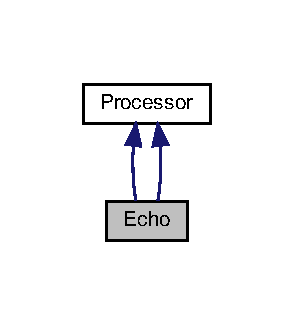
\includegraphics[width=141pt]{classEcho__inherit__graph}
\end{center}
\end{figure}


Collaboration diagram for Echo\+:\nopagebreak
\begin{figure}[H]
\begin{center}
\leavevmode
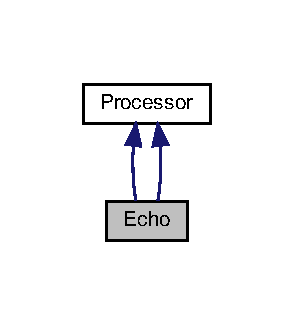
\includegraphics[width=141pt]{classEcho__coll__graph}
\end{center}
\end{figure}
\subsection*{Public Member Functions}
\begin{DoxyCompactItemize}
\item 
\hyperlink{classEcho_ababd42898feed0775f5234d53fe9bff1}{Echo} ()
\item 
\hyperlink{classEcho_a28d71de619dda9e6e51567a04bfb60d6}{Echo} (int new\+Delay)
\item 
int \hyperlink{classEcho_a57e19c9232f9bb96ccd78ba4bb68d6c9}{get\+Delay} ()
\item 
void \hyperlink{classEcho_a3096c57223d6f7ce3097d15e8bf4a0ed}{set\+Delay} (int new\+Delay)
\item 
void \hyperlink{classEcho_a472cc906604bcb493c6a6c1227436938}{processor\+MonoE} (int size, unsigned char $\ast$buffer)
\item 
void \hyperlink{classEcho_a92aa2d47f32f5ad0f2cd45121e8d457f}{processor\+StereoE} (int sizeR, int sizeL, unsigned char $\ast$bufferR, unsigned char $\ast$bufferL)
\item 
void \hyperlink{classEcho_a298f9fe12295c578737928544c46be1a}{processor\+MonoS} (int size, short $\ast$buffer)
\item 
void \hyperlink{classEcho_a26ebcc62f7d6be2e3bd4ac1833636549}{processor\+StereoS} (int sizeR, int sizeL, short $\ast$bufferR, short $\ast$bufferL)
\end{DoxyCompactItemize}


\subsection{Detailed Description}
This is an \hyperlink{classEcho}{Echo} class 

\subsection{Constructor \& Destructor Documentation}
\mbox{\Hypertarget{classEcho_ababd42898feed0775f5234d53fe9bff1}\label{classEcho_ababd42898feed0775f5234d53fe9bff1}} 
\index{Echo@{Echo}!Echo@{Echo}}
\index{Echo@{Echo}!Echo@{Echo}}
\subsubsection{\texorpdfstring{Echo()}{Echo()}\hspace{0.1cm}{\footnotesize\ttfamily [1/2]}}
{\footnotesize\ttfamily Echo\+::\+Echo (\begin{DoxyParamCaption}{ }\end{DoxyParamCaption})}

Base Constructor that takes in the delay for the echo \mbox{\Hypertarget{classEcho_a28d71de619dda9e6e51567a04bfb60d6}\label{classEcho_a28d71de619dda9e6e51567a04bfb60d6}} 
\index{Echo@{Echo}!Echo@{Echo}}
\index{Echo@{Echo}!Echo@{Echo}}
\subsubsection{\texorpdfstring{Echo()}{Echo()}\hspace{0.1cm}{\footnotesize\ttfamily [2/2]}}
{\footnotesize\ttfamily Echo\+::\+Echo (\begin{DoxyParamCaption}\item[{int}]{new\+Delay }\end{DoxyParamCaption})}

Constructor that takes in the delay for the echo 
\begin{DoxyParams}{Parameters}
{\em new\+Delay} & \\
\hline
\end{DoxyParams}


\subsection{Member Function Documentation}
\mbox{\Hypertarget{classEcho_a57e19c9232f9bb96ccd78ba4bb68d6c9}\label{classEcho_a57e19c9232f9bb96ccd78ba4bb68d6c9}} 
\index{Echo@{Echo}!get\+Delay@{get\+Delay}}
\index{get\+Delay@{get\+Delay}!Echo@{Echo}}
\subsubsection{\texorpdfstring{get\+Delay()}{getDelay()}}
{\footnotesize\ttfamily int Echo\+::get\+Delay (\begin{DoxyParamCaption}{ }\end{DoxyParamCaption})}

Getter of delay value \mbox{\Hypertarget{classEcho_a472cc906604bcb493c6a6c1227436938}\label{classEcho_a472cc906604bcb493c6a6c1227436938}} 
\index{Echo@{Echo}!processor\+MonoE@{processor\+MonoE}}
\index{processor\+MonoE@{processor\+MonoE}!Echo@{Echo}}
\subsubsection{\texorpdfstring{processor\+Mono\+E()}{processorMonoE()}}
{\footnotesize\ttfamily void Echo\+::processor\+MonoE (\begin{DoxyParamCaption}\item[{int}]{size,  }\item[{unsigned char $\ast$}]{buffer }\end{DoxyParamCaption})\hspace{0.3cm}{\ttfamily [virtual]}}

Audio \hyperlink{classProcessor}{Processor} for Mono E 
\begin{DoxyParams}{Parameters}
{\em size} & -\/ gets size data \\
\hline
{\em buffer} & -\/ gets range for data \\
\hline
\end{DoxyParams}


Implements \hyperlink{classProcessor_aa9742b5df48a3c6442d521ce93012fc1}{Processor}.

\mbox{\Hypertarget{classEcho_a298f9fe12295c578737928544c46be1a}\label{classEcho_a298f9fe12295c578737928544c46be1a}} 
\index{Echo@{Echo}!processor\+MonoS@{processor\+MonoS}}
\index{processor\+MonoS@{processor\+MonoS}!Echo@{Echo}}
\subsubsection{\texorpdfstring{processor\+Mono\+S()}{processorMonoS()}}
{\footnotesize\ttfamily void Echo\+::processor\+MonoS (\begin{DoxyParamCaption}\item[{int}]{size,  }\item[{short $\ast$}]{buffer }\end{DoxyParamCaption})\hspace{0.3cm}{\ttfamily [virtual]}}

Audio \hyperlink{classProcessor}{Processor} for Mono S 
\begin{DoxyParams}{Parameters}
{\em size} & -\/ gets size data \\
\hline
{\em buffer} & -\/ short integer for buffer \\
\hline
\end{DoxyParams}


Implements \hyperlink{classProcessor_a4cf32c9f7e26383490e8fb49defcc287}{Processor}.

\mbox{\Hypertarget{classEcho_a92aa2d47f32f5ad0f2cd45121e8d457f}\label{classEcho_a92aa2d47f32f5ad0f2cd45121e8d457f}} 
\index{Echo@{Echo}!processor\+StereoE@{processor\+StereoE}}
\index{processor\+StereoE@{processor\+StereoE}!Echo@{Echo}}
\subsubsection{\texorpdfstring{processor\+Stereo\+E()}{processorStereoE()}}
{\footnotesize\ttfamily void Echo\+::processor\+StereoE (\begin{DoxyParamCaption}\item[{int}]{sizeR,  }\item[{int}]{sizeL,  }\item[{unsigned char $\ast$}]{bufferR,  }\item[{unsigned char $\ast$}]{bufferL }\end{DoxyParamCaption})\hspace{0.3cm}{\ttfamily [virtual]}}

Audio \hyperlink{classProcessor}{Processor} for Stereo E 
\begin{DoxyParams}{Parameters}
{\em sizeR} & -\/ gets size data for right side \\
\hline
{\em bufferR} & -\/ gets range for data for right side \\
\hline
{\em bufferL} & -\/ gets range for data for left side \\
\hline
{\em sizeL} & -\/ gets size data for left side \\
\hline
\end{DoxyParams}


Implements \hyperlink{classProcessor_a637904e06d0a3b14f9e1e90fe7f3afbd}{Processor}.

\mbox{\Hypertarget{classEcho_a26ebcc62f7d6be2e3bd4ac1833636549}\label{classEcho_a26ebcc62f7d6be2e3bd4ac1833636549}} 
\index{Echo@{Echo}!processor\+StereoS@{processor\+StereoS}}
\index{processor\+StereoS@{processor\+StereoS}!Echo@{Echo}}
\subsubsection{\texorpdfstring{processor\+Stereo\+S()}{processorStereoS()}}
{\footnotesize\ttfamily void Echo\+::processor\+StereoS (\begin{DoxyParamCaption}\item[{int}]{sizeR,  }\item[{int}]{sizeL,  }\item[{short $\ast$}]{bufferR,  }\item[{short $\ast$}]{bufferL }\end{DoxyParamCaption})\hspace{0.3cm}{\ttfamily [virtual]}}

Audio \hyperlink{classProcessor}{Processor} for Stereo E 
\begin{DoxyParams}{Parameters}
{\em sizeR} & -\/ gets size data for right side \\
\hline
{\em bufferR} & -\/ short integer for buffer on right side \\
\hline
{\em bufferL} & -\/ short integer for buffer on left side \\
\hline
{\em sizeL} & -\/ gets size data for left side \\
\hline
\end{DoxyParams}


Implements \hyperlink{classProcessor_ae3fc266daadbedfa947e596d3ff98a7c}{Processor}.

\mbox{\Hypertarget{classEcho_a3096c57223d6f7ce3097d15e8bf4a0ed}\label{classEcho_a3096c57223d6f7ce3097d15e8bf4a0ed}} 
\index{Echo@{Echo}!set\+Delay@{set\+Delay}}
\index{set\+Delay@{set\+Delay}!Echo@{Echo}}
\subsubsection{\texorpdfstring{set\+Delay()}{setDelay()}}
{\footnotesize\ttfamily void Echo\+::set\+Delay (\begin{DoxyParamCaption}\item[{int}]{new\+Delay }\end{DoxyParamCaption})}

Setter of delay value 
\begin{DoxyParams}{Parameters}
{\em new\+Delay} & \\
\hline
\end{DoxyParams}


The documentation for this class was generated from the following files\+:\begin{DoxyCompactItemize}
\item 
\hyperlink{echo_8h}{echo.\+h}\item 
\hyperlink{echo_8cpp}{echo.\+cpp}\end{DoxyCompactItemize}

\hypertarget{classLimiter}{}\section{Limiter Class Reference}
\label{classLimiter}\index{Limiter@{Limiter}}


{\ttfamily \#include $<$Normalizer.\+h$>$}



Inheritance diagram for Limiter\+:
% FIG 0


Collaboration diagram for Limiter\+:
% FIG 1
\subsection*{Public Member Functions}
\begin{DoxyCompactItemize}
\item 
void \hyperlink{classLimiter_a7be62b79837918824c5a9c52b215d03d}{process\+Buffer} (unsigned char $\ast$buffer, int buffer\+Size) override
\end{DoxyCompactItemize}


\subsection{Detailed Description}
This is a \hyperlink{classLimiter}{Limiter} class 

\subsection{Member Function Documentation}
\mbox{\Hypertarget{classLimiter_a7be62b79837918824c5a9c52b215d03d}\label{classLimiter_a7be62b79837918824c5a9c52b215d03d}} 
\index{Limiter@{Limiter}!process\+Buffer@{process\+Buffer}}
\index{process\+Buffer@{process\+Buffer}!Limiter@{Limiter}}
\subsubsection{\texorpdfstring{process\+Buffer()}{processBuffer()}}
{\footnotesize\ttfamily void Limiter\+::process\+Buffer (\begin{DoxyParamCaption}\item[{unsigned char $\ast$}]{buffer,  }\item[{int}]{buffer\+Size }\end{DoxyParamCaption})\hspace{0.3cm}{\ttfamily [override]}, {\ttfamily [virtual]}}

Process Buffer 
\begin{DoxyParams}{Parameters}
{\em buffer\+Size} & -\/ (insert information about the size) \\
\hline
{\em buffer} & -\/ (insert information about buffer) \\
\hline
\end{DoxyParams}


Implements \hyperlink{classProcessor_a401e57b59e43de9c4a51ca0f566d2948}{Processor}.



The documentation for this class was generated from the following files\+:\begin{DoxyCompactItemize}
\item 
Normalizer.\+h\item 
Normalizer.\+cpp\end{DoxyCompactItemize}

\hypertarget{classNoise__Gate}{}\section{Noise\+\_\+\+Gate Class Reference}
\label{classNoise__Gate}\index{Noise\+\_\+\+Gate@{Noise\+\_\+\+Gate}}


{\ttfamily \#include $<$Noise\+\_\+\+Gate.\+h$>$}



Inheritance diagram for Noise\+\_\+\+Gate\+:
% FIG 0


Collaboration diagram for Noise\+\_\+\+Gate\+:
% FIG 1
\subsection*{Public Member Functions}
\begin{DoxyCompactItemize}
\item 
\hyperlink{classNoise__Gate_a125399a743791634f60e0d1425d79e35}{Noise\+\_\+\+Gate} (int threshold)
\item 
void \hyperlink{classNoise__Gate_a1b30bc5ccc45774528a8f44ba0632291}{process\+Buffer} (unsigned char $\ast$buffer, int buffer\+Size) override
\end{DoxyCompactItemize}


\subsection{Detailed Description}
This is a Noise Gate class 

\subsection{Constructor \& Destructor Documentation}
\mbox{\Hypertarget{classNoise__Gate_a125399a743791634f60e0d1425d79e35}\label{classNoise__Gate_a125399a743791634f60e0d1425d79e35}} 
\index{Noise\+\_\+\+Gate@{Noise\+\_\+\+Gate}!Noise\+\_\+\+Gate@{Noise\+\_\+\+Gate}}
\index{Noise\+\_\+\+Gate@{Noise\+\_\+\+Gate}!Noise\+\_\+\+Gate@{Noise\+\_\+\+Gate}}
\subsubsection{\texorpdfstring{Noise\+\_\+\+Gate()}{Noise\_Gate()}}
{\footnotesize\ttfamily Noise\+\_\+\+Gate\+::\+Noise\+\_\+\+Gate (\begin{DoxyParamCaption}\item[{int}]{threshold }\end{DoxyParamCaption})}

Constructor that takes in the threshold of the Noise Gate 

\subsection{Member Function Documentation}
\mbox{\Hypertarget{classNoise__Gate_a1b30bc5ccc45774528a8f44ba0632291}\label{classNoise__Gate_a1b30bc5ccc45774528a8f44ba0632291}} 
\index{Noise\+\_\+\+Gate@{Noise\+\_\+\+Gate}!process\+Buffer@{process\+Buffer}}
\index{process\+Buffer@{process\+Buffer}!Noise\+\_\+\+Gate@{Noise\+\_\+\+Gate}}
\subsubsection{\texorpdfstring{process\+Buffer()}{processBuffer()}}
{\footnotesize\ttfamily void Noise\+\_\+\+Gate\+::process\+Buffer (\begin{DoxyParamCaption}\item[{unsigned char $\ast$}]{buffer,  }\item[{int}]{buffer\+Size }\end{DoxyParamCaption})\hspace{0.3cm}{\ttfamily [override]}, {\ttfamily [virtual]}}

Process Buffer 
\begin{DoxyParams}{Parameters}
{\em buffer\+Size} & -\/ (insert information about the size) \\
\hline
{\em buffer} & -\/ (insert information about buffer) \\
\hline
\end{DoxyParams}


Implements \hyperlink{classProcessor_a401e57b59e43de9c4a51ca0f566d2948}{Processor}.



The documentation for this class was generated from the following files\+:\begin{DoxyCompactItemize}
\item 
Noise\+\_\+\+Gate.\+h\item 
Noise\+\_\+\+Gate.\+cpp\end{DoxyCompactItemize}

\hypertarget{classProcessor}{}\section{Processor Class Reference}
\label{classProcessor}\index{Processor@{Processor}}


{\ttfamily \#include $<$Processor.\+h$>$}



Inheritance diagram for Processor\+:
% FIG 0
\subsection*{Public Member Functions}
\begin{DoxyCompactItemize}
\item 
virtual void \hyperlink{classProcessor_a401e57b59e43de9c4a51ca0f566d2948}{process\+Buffer} (unsigned char $\ast$buffer, int buffer\+Size)=0
\end{DoxyCompactItemize}


\subsection{Detailed Description}
This is a \hyperlink{classProcessor}{Processor} class 

\subsection{Member Function Documentation}
\mbox{\Hypertarget{classProcessor_a401e57b59e43de9c4a51ca0f566d2948}\label{classProcessor_a401e57b59e43de9c4a51ca0f566d2948}} 
\index{Processor@{Processor}!process\+Buffer@{process\+Buffer}}
\index{process\+Buffer@{process\+Buffer}!Processor@{Processor}}
\subsubsection{\texorpdfstring{process\+Buffer()}{processBuffer()}}
{\footnotesize\ttfamily virtual void Processor\+::process\+Buffer (\begin{DoxyParamCaption}\item[{unsigned char $\ast$}]{buffer,  }\item[{int}]{buffer\+Size }\end{DoxyParamCaption})\hspace{0.3cm}{\ttfamily [pure virtual]}}

Process Buffer 
\begin{DoxyParams}{Parameters}
{\em buffer\+Size} & -\/ (insert information about the size) \\
\hline
{\em buffer} & -\/ (insert information about buffer) \\
\hline
\end{DoxyParams}


Implemented in \hyperlink{classNoise__Gate_a1b30bc5ccc45774528a8f44ba0632291}{Noise\+\_\+\+Gate}, and \hyperlink{classLimiter_a7be62b79837918824c5a9c52b215d03d}{Limiter}.



The documentation for this class was generated from the following file\+:\begin{DoxyCompactItemize}
\item 
Processor.\+h\end{DoxyCompactItemize}

\hypertarget{structWave__Header}{}\section{Wave\+\_\+\+Header Struct Reference}
\label{structWave__Header}\index{Wave\+\_\+\+Header@{Wave\+\_\+\+Header}}
\subsection*{Public Attributes}
\begin{DoxyCompactItemize}
\item 
\mbox{\Hypertarget{structWave__Header_ac90ed5a284cbf30b3f69ea082de3a0c6}\label{structWave__Header_ac90ed5a284cbf30b3f69ea082de3a0c6}} 
char {\bfseries riff} \mbox{[}4\mbox{]}
\item 
\mbox{\Hypertarget{structWave__Header_a6928c2d8b8904339ebb788eb8290f142}\label{structWave__Header_a6928c2d8b8904339ebb788eb8290f142}} 
int {\bfseries wav\+Size}
\item 
\mbox{\Hypertarget{structWave__Header_a0619c4f802e42c1f0df93f77eab026b3}\label{structWave__Header_a0619c4f802e42c1f0df93f77eab026b3}} 
char {\bfseries wave} \mbox{[}4\mbox{]}
\item 
\mbox{\Hypertarget{structWave__Header_a14d810235149a0b8bfab223852e1d414}\label{structWave__Header_a14d810235149a0b8bfab223852e1d414}} 
char {\bfseries fmt} \mbox{[}4\mbox{]}
\item 
\mbox{\Hypertarget{structWave__Header_a6b4c3112066ec18881997ca2f42b9c53}\label{structWave__Header_a6b4c3112066ec18881997ca2f42b9c53}} 
int {\bfseries fmt\+Chunk\+Size}
\item 
\mbox{\Hypertarget{structWave__Header_a78581f9b4fa8ccd937260f6acd1805e4}\label{structWave__Header_a78581f9b4fa8ccd937260f6acd1805e4}} 
short {\bfseries audio\+Format}
\item 
\mbox{\Hypertarget{structWave__Header_a06db23d3c3ae3e20dca44ec8e1b62210}\label{structWave__Header_a06db23d3c3ae3e20dca44ec8e1b62210}} 
short {\bfseries num\+Channels}
\item 
\mbox{\Hypertarget{structWave__Header_ab5fb0a7055f8ea82df946d215bc803ee}\label{structWave__Header_ab5fb0a7055f8ea82df946d215bc803ee}} 
int {\bfseries sample\+Rate}
\item 
\mbox{\Hypertarget{structWave__Header_ad060843c06006ec4158afc8dccea9fc3}\label{structWave__Header_ad060843c06006ec4158afc8dccea9fc3}} 
int {\bfseries byte\+Rate}
\item 
\mbox{\Hypertarget{structWave__Header_aa9440351df7a8f57a5536fea94958c56}\label{structWave__Header_aa9440351df7a8f57a5536fea94958c56}} 
short {\bfseries sample\+Alignment}
\item 
\mbox{\Hypertarget{structWave__Header_a84a83027dfbce3d40ef313e2e51fb14c}\label{structWave__Header_a84a83027dfbce3d40ef313e2e51fb14c}} 
short {\bfseries bit\+Depth}
\item 
\mbox{\Hypertarget{structWave__Header_a4e2bc40c58a9da8bbe53b14e9f822153}\label{structWave__Header_a4e2bc40c58a9da8bbe53b14e9f822153}} 
char {\bfseries data\+\_\+header} \mbox{[}4\mbox{]}
\item 
\mbox{\Hypertarget{structWave__Header_a30a52cd01475ca214d183dfb1d6c4230}\label{structWave__Header_a30a52cd01475ca214d183dfb1d6c4230}} 
int {\bfseries data\+\_\+bytes}
\end{DoxyCompactItemize}


The documentation for this struct was generated from the following file\+:\begin{DoxyCompactItemize}
\item 
Wave\+\_\+\+Header.\+h\end{DoxyCompactItemize}

\chapter{File Documentation}
\hypertarget{main_8cpp}{}\section{main.\+cpp File Reference}
\label{main_8cpp}\index{main.\+cpp@{main.\+cpp}}
{\ttfamily \#include $<$iostream$>$}\newline
{\ttfamily \#include $<$fstream$>$}\newline
{\ttfamily \#include $<$string$>$}\newline
{\ttfamily \#include $<$vector$>$}\newline
{\ttfamily \#include \char`\"{}Wave\+\_\+\+Header.\+h\char`\"{}}\newline
Include dependency graph for main.\+cpp\+:

%--- End generated contents ---

% Index
\backmatter
\newpage
\phantomsection
\clearemptydoublepage
\addcontentsline{toc}{chapter}{Index}
\printindex

\end{document}
